% ============================================================================
%  Rapport — Partie 1 : isoler la longueur du texte
%  Compilation : pdflatex -> bibtex -> pdflatex -> pdflatex
%  (bibliographie : references.bib, partagee avec le reste du rapport)
%  Les figures sont produites par :
%      python report/figures/make_isolation_figures.py
%  à partir de results/block_duel/block_duel.json et
%           de results/comet_align/comet_align.json
%  Si babel-french est installé, décommenter la ligne \usepackage[french]{babel}
%  pour obtenir la typographie française automatique.
% ============================================================================
\documentclass[11pt]{article}
\usepackage[a4paper,margin=2.5cm]{geometry}
\usepackage[T1]{fontenc}
\usepackage[utf8]{inputenc}
\usepackage{lmodern}
% \usepackage[french]{babel}
\usepackage{booktabs}
\usepackage{graphicx}
\usepackage{amsmath}
\usepackage{amssymb}
\usepackage{multirow}
\usepackage{caption}
\usepackage{tikz}
\usetikzlibrary{positioning,decorations.pathreplacing}
\usepackage[round]{natbib}
\usepackage[hidelinks]{hyperref}
\usepackage{xcolor}

\captionsetup{font=small,labelfont=bf}
\graphicspath{{figures/}{figures/isolation/}}

\newcommand{\cometda}{\textsc{wmt22-comet-da}}
\newcommand{\kiwi}{\textsc{wmt22-cometkiwi-da}}
\newcommand{\code}[1]{\texttt{\small #1}}

\title{Partie 1 --- Isoler la longueur du texte\\
\large Alignement de blocs FLORES+ avec un seul distracteur perturbé}
\author{Adle Ben Salem \\ \small Inria Paris}
\date{Septembre 2026 --- rapport de travail}

\begin{document}
\maketitle

\section{Question et principe}

Les métriques apprises comme COMET sont entraînées sur des phrases isolées.
Elles sont appliquées à des paragraphes et à des documents.
Nous voulons savoir ce que coûte cet écart.

La difficulté est que « texte plus long » veut dire plusieurs choses à la fois.
Un texte long contient plus de contenu, plus de sujets, plus de candidats possibles.
Nous voulons donc une expérience où la longueur est la \emph{seule} variable qui change.

Le principe est simple.
Nous prenons $k$ phrases consécutives d'un même article et nous les concaténons.
Nous obtenons un \emph{bloc}.
Nous injectons \emph{une} erreur dans \emph{une} phrase du bloc.
Nous demandons au modèle de retrouver le bloc correct.
Quand $k$ augmente, l'erreur reste la même mais le texte autour grandit.
L'erreur est diluée.
C'est cette dilution que nous mesurons.

Le protocole est une transposition de xSIM++ \citep{chen2023xsimpp} au niveau du bloc.
xSIM++ perturbe une phrase et mesure si un encodeur préfère toujours la bonne traduction.
Nous gardons ses trois catégories de perturbation et nous ajoutons la longueur comme variable contrôlée.

\paragraph{Vocabulaire.}
Nous employons les mêmes mots dans tout le rapport (tableau~\ref{tab:vocab}).
En particulier, nous n'écrivons jamais « $P$(gold beats the negative) ».
Nous écrivons soit le \emph{taux de réussite de l'alignement}, soit le \emph{rang moyen de la référence}.

\begin{table}[t]
\centering\small
\begin{tabular}{p{4.1cm} p{10.3cm}}
\toprule
terme & définition employée dans ce rapport\\
\midrule
phrase & une ligne de FLORES+, alignée dans toutes les langues\\
article & le document source d'où vient la phrase (identifié par son URL)\\
bloc & $k$ phrases consécutives d'un même article, concaténées dans l'ordre\\
position & l'indice de la phrase dans le bloc, de $1$ à $k$\\
bloc source & le bloc en anglais ; c'est la requête\\
bloc de référence & le bloc formé des $k$ traductions correctes ; c'est la bonne réponse\\
perturbation & une édition locale d'une seule phrase : causalité, entité ou nombre\\
distracteur & un bloc de référence dont \emph{une} phrase a été perturbée\\
$D$ & le nombre de distracteurs présentés à chaque décision\\
taux de réussite & part des décisions où la référence obtient le meilleur score\\
rang moyen & rang de la référence parmi les $D+1$ candidats, $1$ = meilleur\\
\bottomrule
\end{tabular}
\caption{Terminologie. Un « distracteur » est toujours une copie perturbée du bloc de référence lui-même, jamais la traduction d'un autre article.}
\label{tab:vocab}
\end{table}

\section{Données : FLORES+}

\subsection{Le corpus}

FLORES+ est un corpus de traduction \emph{multiparallèle} \citep{nllb2022,goyal2022flores,oldi2024flores}.
La même phrase source est traduite dans plus de 200 langues.
Les phrases proviennent d'articles de Wikinews, Wikijunior et Wikivoyage.
Chaque ligne porte l'URL de son article d'origine.

Deux propriétés nous intéressent.

Premièrement, l'alignement est ligne à ligne.
La ligne $i$ en anglais et la ligne $i$ en français sont la même phrase.
Concaténer les lignes $i$ à $i+k-1$ dans deux langues produit donc deux blocs qui se correspondent exactement.

Deuxièmement, les lignes consécutives d'un même article forment un texte cohérent.
Un bloc n'est pas un sac de phrases sans rapport.
C'est un extrait de document réel.

Nous utilisons les partitions \code{dev} (997 phrases) et \code{devtest} (1012 phrases).
Cela fait \textbf{2009 phrases alignées par langue}.

\subsection{Langues et direction}

Nous étudions quatre langues cibles : \textbf{allemand (de), espagnol (es), français (fr) et russe (ru)}.
La source est toujours l'\textbf{anglais}.
Nous n'évaluons donc que la direction en$\to$xx, soit quatre paires : en--de, en--es, en--fr, en--ru.
Aucune paire sans anglais n'est évaluée : l'anglais est le pivot et sert toujours de requête.
Le code accepte aussi \code{--direction xx2en}, mais cette option n'a pas été utilisée pour les résultats présentés ici.

Le chinois est possible avec le générateur de perturbations spaCy, qui sait détecter des entités dans une écriture sans casse.
Le chinois a servi dans un essai préliminaire à petite échelle, mais il ne figure pas dans les mesures présentées ici.

\subsection{Construction des blocs}

Un bloc est construit par une fenêtre glissante sur les lignes, avec trois contraintes.

\begin{enumerate}
\item \textbf{Les blocs ne traversent pas un article.} Une fenêtre qui rencontre un changement d'URL est abandonnée.
\item \textbf{Les blocs ne se recouvrent pas.} Le pas vaut $k$. Deux blocs voisins ne partagent aucune phrase. Des fenêtres recouvrantes mettraient des quasi-doublons dans le jeu de candidats, ce qui est un autre problème, et un problème confondu.
\item \textbf{Le même découpage sert dans toutes les langues.} Les lignes étant alignées, un bloc est défini par des indices de lignes, pas par du texte. Le bloc source et le bloc de référence couvrent donc exactement les mêmes phrases, dans deux langues différentes.
\end{enumerate}

Le séparateur de concaténation est l'espace, sauf pour les langues sans espace (zh, ja, th) où il est vide.

La figure~\ref{fig:flores} illustre la construction.
Le tableau~\ref{tab:donnees} donne les quantités obtenues, et la figure~\ref{fig:donnees} en donne une vue graphique.
Le nombre de blocs chute vite : à $k=5$ il ne reste que 141 blocs par langue, soit 35~\% du maximum théorique $\lfloor 2009/5 \rfloor$.
La raison est la contrainte d'article : les articles de FLORES+ sont courts, donc peu d'entre eux fournissent cinq lignes consécutives complètes.
C'est une limite du corpus, pas du protocole, et elle impose de lire les points à grand $k$ avec prudence.

% ---------------------------------------------------------------- figure TikZ
\begin{figure}[t]
\centering
\resizebox{\linewidth}{!}{%
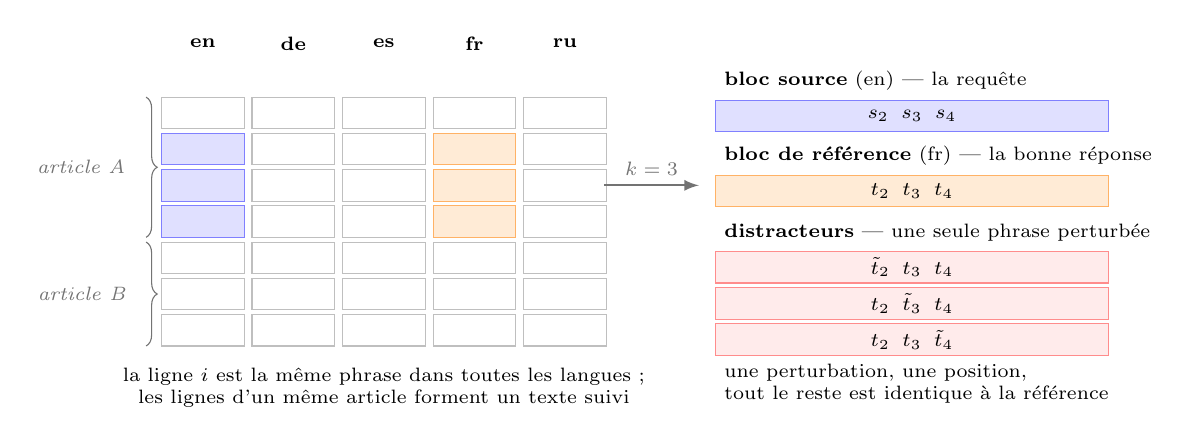
\begin{tikzpicture}[
  cell/.style={draw=black!25, fill=white, minimum width=1.05cm,
               minimum height=0.40cm, inner sep=0pt},
  src/.style={cell, fill=blue!12, draw=blue!50},
  ref/.style={cell, fill=orange!16, draw=orange!60},
  neg/.style={cell, fill=red!8, draw=red!45},
  hd/.style={font=\scriptsize\bfseries},
  tx/.style={font=\scriptsize},
  ty/.style={font=\scriptsize\itshape}
]
% ---- colonnes = langues, lignes = phrases -------------------------------
\foreach \l [count=\i from 0] in {en,de,es,fr,ru}
  \node[hd] at (\i*1.15, 0.42) {\l};
\foreach \r in {1,...,7}
  \foreach \i in {0,...,4}
    \node[cell] at (\i*1.15, -\r*0.46) {};
% blocs surlignes : lignes 2-4, colonnes en et fr
\foreach \r in {2,3,4}{
  \node[src] at (0, -\r*0.46) {};
  \node[ref] at (3*1.15, -\r*0.46) {};
}
% accolades d'articles
\draw[decorate, decoration={brace, amplitude=4pt}, black!55]
  (-0.72,-0.26) -- (-0.72,-2.04) node[midway, left=4pt, ty] {article A};
\draw[decorate, decoration={brace, amplitude=4pt}, black!55]
  (-0.72,-2.10) -- (-0.72,-3.42) node[midway, left=4pt, ty] {article B};
\node[tx, align=center] at (2.3, -3.95)
  {la ligne $i$ est la même phrase dans toutes les langues ;\\
   les lignes d'un même article forment un texte suivi};

% ---- fleche ------------------------------------------------------------
\draw[-latex, black!55, thick] (5.1,-1.38) -- (6.3,-1.38)
  node[midway, above, ty] {$k=3$};

% ---- blocs construits --------------------------------------------------
\node[tx, anchor=west] at (6.5,-0.05) {\textbf{bloc source} (en) --- la requête};
\node[src, minimum width=5.0cm, anchor=west] at (6.5,-0.50)
  {\scriptsize $s_2 \;\; s_3 \;\; s_4$};

\node[tx, anchor=west] at (6.5,-1.00) {\textbf{bloc de référence} (fr) --- la bonne réponse};
\node[ref, minimum width=5.0cm, anchor=west] at (6.5,-1.45)
  {\scriptsize $t_2 \;\; t_3 \;\; t_4$};

\node[tx, anchor=west] at (6.5,-1.98) {\textbf{distracteurs} --- une seule phrase perturbée};
\node[neg, minimum width=5.0cm, anchor=west] at (6.5,-2.42)
  {\scriptsize $\tilde t_2 \;\; t_3 \;\; t_4$};
\node[neg, minimum width=5.0cm, anchor=west] at (6.5,-2.88)
  {\scriptsize $t_2 \;\; \tilde t_3 \;\; t_4$};
\node[neg, minimum width=5.0cm, anchor=west] at (6.5,-3.34)
  {\scriptsize $t_2 \;\; t_3 \;\; \tilde t_4$};
\node[tx, anchor=west, align=left] at (6.5,-3.90)
  {une perturbation, une position,\\ tout le reste est identique à la référence};
\end{tikzpicture}}
\caption{Construction des blocs. À gauche, FLORES+ : les colonnes sont les langues, les lignes sont les phrases, et les lignes consécutives d'un même article forment un texte suivi. À droite, un bloc de $k=3$ phrases. Le bloc source est la requête. Le bloc de référence est la concaténation des trois traductions correctes. Chaque distracteur ne diffère de la référence que par une seule phrase, notée $\tilde t$.}
\label{fig:flores}
\end{figure}

\begin{table}[t]
\centering\small
\begin{tabular}{l rrrrr}
\toprule
& \multicolumn{5}{c}{phrases par bloc}\\
\cmidrule(lr){2-6}
& $k{=}1$ & $k{=}2$ & $k{=}3$ & $k{=}4$ & $k{=}5$\\
\midrule
maximum théorique $\lfloor 2009/k \rfloor$   & 2\,009 & 1\,004 & 669 & 502 & 401\\
blocs construits, par langue                 & 2\,009 & 846 & 468 & 276 & 141\\
blocs construits, 4 langues                  & 8\,036 & 3\,384 & 1\,872 & 1\,104 & 564\\
distracteurs possibles par bloc ($\le 3k$)   & 3 & 6 & 9 & 12 & 15\\
\midrule
\multicolumn{6}{l}{\emph{blocs perturbés produits, 4 langues (au plus deux variantes par position et catégorie)}}\\
\quad causalité & 13\,370 & 11\,246 & 9\,347 & 7\,343 & 4\,664\\
\quad entité    & 8\,774  & 7\,478  & 6\,032 & 4\,862 & 2\,866\\
\quad nombre    & 4\,380  & 3\,748  & 3\,094 & 2\,462 & 1\,366\\
\midrule
\multicolumn{6}{l}{\emph{couverture : part des blocs offrant au moins $D$ distracteurs}}\\
\quad $D=2$ & .87 & 1.00 & 1.00 & 1.00 & 1.00\\
\quad $D=4$ & --- & .41 & .60 & .79 & .84\\
\quad $D=5$ & --- & .14 & .47 & .63 & .72\\
\quad $D=6$ & --- & .03 & .37 & .51 & .62\\
\midrule
\multicolumn{6}{l}{\emph{nombre de décisions effectivement notées, 4 langues}}\\
\quad $D=2$ & 7\,027 & 3\,379 & 1\,872 & 1\,104 & 564\\
\quad $D=4$ & --- & 1\,376 & 1\,132 & 867 & 474\\
\quad $D=5$ & --- & 457 & 884 & 697 & 407\\
\quad $D=6$ & --- & 103 & 685 & 565 & 349\\
\bottomrule
\end{tabular}
\caption{Le corpus de blocs. Le nombre de blocs est le même dans les quatre langues, puisqu'un bloc est défini par des indices de lignes. Les comptes de blocs perturbés correspondent au vivier construit avec deux variantes par (position, catégorie) ; le protocole du duel, lui, n'en garde qu'une, d'où la borne $3k$. Un $D$ élevé à petit $k$ ne retient qu'une minorité de blocs : à $k{=}2$ et $D{=}6$, seuls 3~\% des blocs sont éligibles.}
\label{tab:donnees}
\end{table}

\begin{figure}[t]
\centering
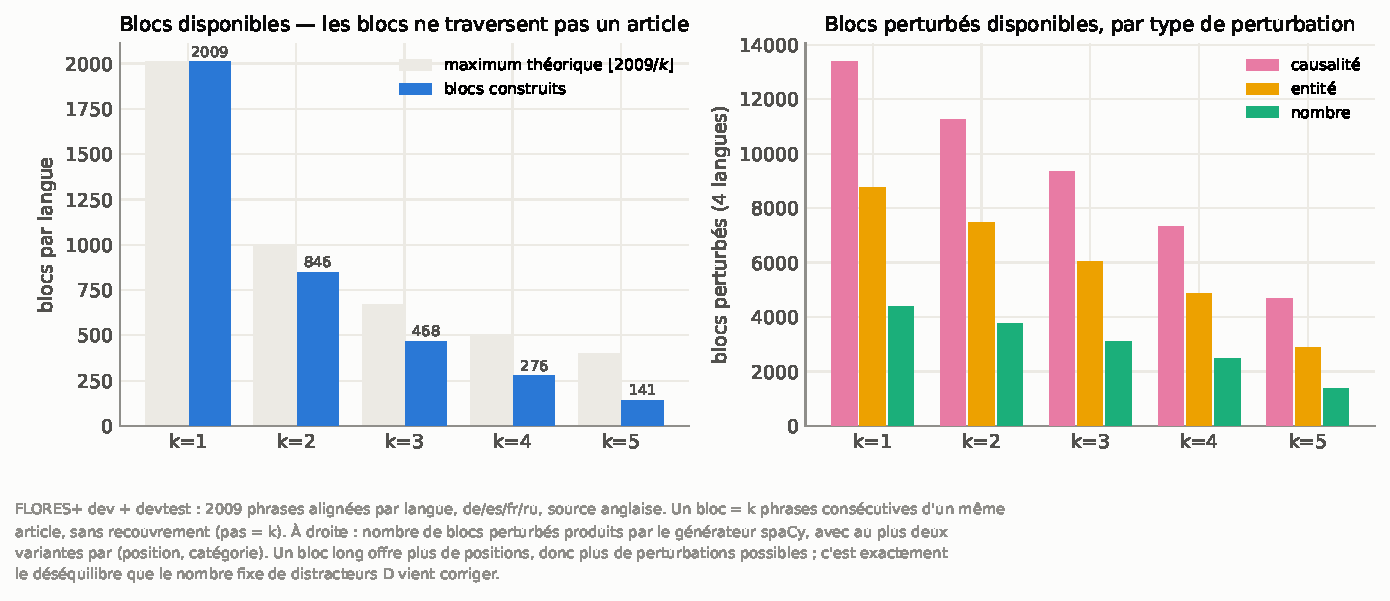
\includegraphics[width=\linewidth]{iso_data.pdf}
\caption{Le corpus de blocs, vu autrement. À gauche : le nombre de blocs s'effondre quand $k$ augmente, parce que les articles de FLORES+ sont courts. À droite : le nombre de blocs perturbés disponibles par catégorie. La causalité est presque toujours applicable ; le nombre l'est trois fois moins souvent.}
\label{fig:donnees}
\end{figure}

\section{Les perturbations}

\subsection{Les trois catégories}

Nous reprenons exactement les trois catégories de xSIM++ \citep{chen2023xsimpp}.

\begin{description}
\item[causalité] Le sens est inversé ou durci : antonyme, négation ajoutée ou retirée, modalité renforcée.
\item[entité] Une entité nommée est remplacée par une autre entité du corpus.
\item[nombre] Une valeur numérique ou un ordinal est remplacé par une autre valeur.
\end{description}

Une différence avec l'article d'origine mérite d'être notée.
xSIM++ perturbe le côté \emph{anglais}.
Ici la perturbation porte sur le côté \emph{cible}, c'est-à-dire sur la traduction, puisque c'est la traduction que le modèle doit retrouver.
Les perturbations sont donc appliquées en allemand, espagnol, français et russe, et non en anglais.

\subsection{Comment chaque perturbation est produite}

Le générateur par défaut s'appuie sur spaCy \citep{honnibal2020spacy} : une analyse morphosyntaxique, une reconnaissance d'entités nommées et un arbre de dépendances par langue.
Les modèles utilisés sont les petits modèles officiels : \code{de\_core\_news\_sm}, \code{es\_core\_news\_sm}, \code{fr\_core\_news\_sm}, \code{ru\_core\_news\_sm}.
Le corpus entier est analysé une fois, puis deux banques sont constituées par langue :
la \emph{banque d'entités}, qui contient toutes les entités nommées vues dans le corpus, rangées par type ;
et la \emph{banque de numéraux}, qui contient les cardinaux et les ordinaux écrits en toutes lettres.

La figure~\ref{fig:pseudo} donne la procédure complète en pseudo-code.
Les trois paragraphes qui suivent la détaillent.

\paragraph{Nombre.}
On collecte dans la phrase tous les tokens qui contiennent un chiffre, tous les tokens dont l'étiquette est \code{NUM} et qui ressemblent à un nombre, et tous les ordinaux (trait \code{NumType=Ord} ou appartenance à la liste d'ordinaux de la langue).
On en tire un au hasard.
Si le token contient des chiffres, la suite de chiffres est remplacée par une autre suite \emph{de même longueur} ; « 1998 » devient « 3471 », jamais « 34 ».
Cette contrainte évite qu'une différence de longueur visible ne trahisse la perturbation.
Sinon, le mot est remplacé par un autre élément de la banque, ordinal contre ordinal et cardinal contre cardinal, en conservant la casse initiale.

\paragraph{Entité.}
On collecte les entités nommées de la phrase dont le type appartient à une liste fermée : personnes, lieux, organisations, événements, produits, œuvres, nationalités.
Les types numériques de spaCy (\code{CARDINAL}, \code{ORDINAL}, \code{DATE}, \code{PERCENT}, \code{MONEY}, \code{QUANTITY}) sont \emph{exclus} : ils appartiennent à la catégorie nombre, et laisser deux catégories modifier le même empan rendrait la comparaison entre catégories illisible.
Une entité précédée d'une apostrophe est également écartée, car l'élision rendrait le résultat agrammatical (« l'université Stanford » $\to$ « l'Berlin »).
On tire une entité au hasard et on la remplace par une entité \emph{du même type} tirée de la banque ; si aucune n'est disponible, par une entité de n'importe quel type.

\paragraph{Causalité.}
Trois opérations sont tentées dans un ordre tiré au hasard, et la première qui produit un texte différent est retenue.
\emph{Antonyme} : un mot du lexique d'antonymes de la langue est remplacé par son contraire ; en anglais seulement, WordNet \citep{miller1995wordnet} est consulté en second recours, et uniquement lorsque la forme de surface est déjà le lemme.
\emph{Renforcement modal} : un modal prudent devient un modal assertif (« pourrait » $\to$ « va », « peut » $\to$ « doit »).
\emph{Négation} : si la phrase contient déjà une négation, elle est supprimée ; sinon une négation est insérée sur le verbe fini.
La suppression s'appuie sur l'analyse en dépendances, ce qui compte : en français, « ne \ldots{} pas » est retiré \emph{en entier}, car retirer une seule des deux particules n'inverse rien.
L'insertion respecte l'ordre des mots de la langue : « nicht » se place après le verbe fini en allemand, « no » avant le verbe et avant les clitiques en espagnol, « ne \ldots{} pas » encadre le verbe en français avec élision (« n'a pas »).

\begin{figure}[t]
\small
\hrule\vspace{4pt}
\begin{verbatim}
perturber(phrase, categorie, graine) :
    rng <- generateur aleatoire seme par (graine, langue, categorie, phrase, i)

    si categorie = "nombre" :
        cibles <- tokens contenant un chiffre
                  + tokens NUM ressemblant a un nombre
                  + ordinaux (NumType=Ord ou liste de la langue)
        si cibles vide : retourner AUCUNE
        t <- rng.choix(cibles)
        si t contient des chiffres :
            remplacer la suite de chiffres par une autre de MEME longueur
        sinon :
            remplacer t par un autre element de la banque (ordinal / cardinal)

    si categorie = "entite" :
        cibles <- entites nommees de type PER/LOC/GPE/ORG/EVENT/...
                  (types numeriques exclus, elision exclue)
        si cibles vide : retourner AUCUNE
        e <- rng.choix(cibles)
        remplacer e par une autre entite du MEME type, tiree de la banque

    si categorie = "causalite" :
        pour op dans rng.melange(["antonyme", "modal", "negation"]) :
            antonyme : lexique de la langue, puis WordNet (anglais seulement)
            modal    : modal prudent -> modal assertif
            negation : si negation presente -> la supprimer en entier
                       sinon -> l'inserer sur le verbe fini
            si le resultat differe de la phrase : le retourner

    retourner AUCUNE   # la phrase n'admet pas cette perturbation
\end{verbatim}
\vspace{2pt}\hrule
\caption{Génération d'une perturbation. La fonction renvoie \code{AUCUNE} quand la phrase ne s'y prête pas : une phrase sans chiffre ni ordinal n'admet pas de perturbation « nombre ». Le générateur est réessayé avec un indice de variante $i$ différent tant que le nombre de variantes demandé n'est pas atteint.}
\label{fig:pseudo}
\end{figure}

\subsection{Deux propriétés qui rendent la comparaison entre longueurs valide}

\paragraph{Déterminisme.}
Le générateur aléatoire est semé par le quintuplet
\[
(\text{graine},\ \text{langue},\ \text{catégorie},\ \text{texte de la phrase},\ \text{indice de variante}).
\]
La graine vaut 42 dans toutes nos exécutions.
Rien dans cette clé ne dépend de $k$, ni de la position de la phrase, ni du bloc.

\paragraph{Emboîtement des perturbations.}
La conséquence est directe et importante.
Une phrase donnée reçoit toujours la \emph{même} perturbation, quel que soit le bloc qui la contient.
Les blocs de taille $k+1$ portent donc, aux positions $1, \dots, k$, exactement les mêmes perturbations que les blocs de taille $k$.
Passer de $k$ à $k+1$ n'ajoute qu'une chose : du texte non perturbé autour de l'erreur.
C'est ce qui permet d'attribuer à la longueur, et à elle seule, la variation observée.

\paragraph{Une perturbation par position et par catégorie.}
Pour le protocole principal, nous ne gardons qu'\emph{une} variante par couple (position, catégorie).
Un bloc de $k$ phrases admet donc au plus $m \le 3k$ distracteurs.
Le maximum n'est presque jamais atteint : une phrase sans chiffre n'admet pas de perturbation « nombre », une phrase sans entité nommée n'admet pas de perturbation « entité ».
Le tableau~\ref{tab:donnees} montre ce déséquilibre : la causalité est presque toujours applicable, le nombre l'est trois fois moins souvent.

\section{La tâche d'alignement}

\subsection{Ce qui est demandé au modèle}

Une décision se présente ainsi.
La requête est le bloc source en anglais.
Les candidats sont le bloc de référence dans la langue cible, plus $D$ distracteurs.
Le modèle attribue un score à chaque candidat.
Il réussit s'il donne le meilleur score à la référence.

\subsection{Le jeu de candidats}

Les distracteurs sont les copies perturbées \textbf{du bloc de référence lui-même}, à différentes positions et avec différentes catégories.
Les blocs de référence des \emph{autres} articles ne sont pas candidats.

Ce choix est délibéré.
Distinguer deux articles est une compétence différente, et une compétence facile.
Un essai de contrôle le vérifie : sur un vivier composé uniquement de blocs corrects, l'erreur d'alignement vaut exactement $0{,}000$ dans les vingt cellules (langue, $k$) mesurées.\footnote{Essai à petite échelle : \code{multilingual-e5-small}, 80 blocs par cellule, cinq langues (de, es, fr, ru, zh). Voir \code{results/block\_xsim\_spacy/}, où les quatre viviers emboîtés sont comparés sur la même matrice de similarité.}
Laisser ces candidats dans le vivier gonfle donc la sensibilité apparente à l'erreur injectée : un modèle peut sembler détecter l'édition alors qu'il reconnaît seulement le sujet.
En les retirant, il ne reste plus que la perturbation à séparer.

\subsection{Pourquoi $D$ doit être fixé}

Un bloc de cinq phrases admet plus de perturbations qu'un bloc de deux phrases.
Si nous présentions tous les distracteurs disponibles, le nombre de candidats croîtrait avec $k$.
La tâche deviendrait mécaniquement plus difficile à grand $k$, indépendamment de la dilution.
La longueur et la difficulté seraient confondues.

Nous fixons donc $D$, le nombre de distracteurs, indépendamment de $k$.
Un bloc qui ne fournit pas $D$ distracteurs est \emph{écarté}, pas complété : le compléter avec un candidat plus facile rendrait cette décision moins coûteuse que les autres et biaiserait la moyenne.
Le nombre de blocs écartés est reporté (tableau~\ref{tab:donnees}).

\subsection{Toutes les manières de tirer $D$ distracteurs}

Un bloc dispose de $m$ distracteurs, avec $m \ge D$.
Il existe $\binom{m}{D}$ manières d'en choisir $D$.
Nous ne tirons pas un sous-ensemble au hasard : nous les évaluons \emph{tous}, et nous moyennons.

Ce calcul a une forme close, ce qui le rend gratuit.
Soit $w$ le nombre de distracteurs du bloc que la référence bat, c'est-à-dire ceux dont le score est strictement inférieur à celui de la référence.
La référence gagne face à un sous-ensemble $S$ si et seulement si elle bat chacun de ses membres.
Le nombre de sous-ensembles gagnants est donc $\binom{w}{D}$, et
\[
\Pr[\text{réussite sur le bloc } b] \;=\; \frac{\binom{w_b}{D}}{\binom{m_b}{D}} .
\]
Aucune énumération n'est nécessaire et la moyenne est exacte.
Une égalité de scores compte contre la référence.

\section{Les deux métriques}

Nous rapportons deux quantités, et deux seulement.

\paragraph{1. Taux de réussite de l'alignement, $A(D)$.}
C'est la part des décisions où la référence obtient le meilleur score parmi les $D+1$ candidats.
En notant $B_D$ l'ensemble des blocs qui fournissent au moins $D$ distracteurs,
\[
A(D) \;=\; \frac{1}{|B_D|} \sum_{b \in B_D} \frac{\binom{w_b}{D}}{\binom{m_b}{D}} ,
\qquad \text{hasard} = \frac{1}{D+1}.
\]
C'est la métrique la plus directe : le modèle a-t-il fait le bon choix, oui ou non.
Elle a un défaut : elle ne distingue pas un échec de peu d'un échec total.

\paragraph{2. Rang moyen de la référence, $R(D)$.}
C'est le rang de la référence dans le classement des $D+1$ candidats par score décroissant, $1$ étant le meilleur.
Il vaut $1$ plus le nombre de distracteurs mieux notés que la référence.
Moyenné sur tous les sous-ensembles de taille $D$, le nombre attendu de distracteurs mieux notés vaut $D\,(m_b-w_b)/m_b$, donc
\[
R(D) \;=\; 1 + \frac{D}{|B_D|} \sum_{b \in B_D} \frac{m_b - w_b}{m_b} ,
\qquad \text{hasard} = \frac{D+2}{2}.
\]
Cette métrique dit \emph{à quel point} le modèle se trompe.
Un rang au-dessus du hasard signifie que le modèle préfère activement les copies perturbées à la traduction correcte.
C'est une information que le taux de réussite seul ne donne pas.

\paragraph{Quantité intermédiaire.}
Nous utilisons aussi le \emph{taux de victoire par paire} : la part des couples (référence, distracteur) où la référence est mieux notée, soit $\bar p = \mathrm{moy}_b\, w_b/m_b$.
C'est la version $D=1$ du taux de réussite.
Elle sert à deux choses : la ventilation par catégorie de perturbation, où elle utilise \emph{tous} les distracteurs disponibles et couvre donc 100~\% des blocs ; et le calcul de $R(D) = 1 + D\,(1-\bar p)$.
Les valeurs de $R$ rapportées au tableau~\ref{tab:principal} sont obtenues par cette formule à partir du taux de victoire par paire agrégé, ce qui suppose ce taux homogène entre blocs d'une même cellule ; le rang exact, calculé décision par décision, est rapporté au tableau~\ref{tab:comet} pour le protocole à $D=2$.

\paragraph{Correspondance avec le code.}
$A(D)$ est \code{1 - by\_duel\_size[D].duel\_err} dans \code{results/block\_duel/block\_duel.json}, et \code{shortlist\_accuracy} dans \code{results/comet\_align/comet\_align.json}.
Le taux de victoire par paire est \code{detection\_rate} dans le premier fichier et \code{duel\_accuracy} dans le second.
Le rang exact est \code{shortlist\_mean\_rank}.

\section{Les modèles comparés}

Nous comparons quatre encodeurs gelés, plus une variante de contrôle.
Aucun n'est entraîné sur la tâche.
Le score d'un candidat est la \textbf{similarité cosinus} entre le plongement du bloc source et le plongement du candidat.
Tous les plongements sont normalisés en norme $L_2$, donc le cosinus est un simple produit scalaire.

\begin{description}
\item[encodeur COMET-DA] \cometda{} \citep{rei2022comet}. Le plongement est celui que COMET calcule lui-même : attention par couche sur toutes les couches, puis moyenne. C'est bien la représentation sur laquelle la tête de régression est posée.
\item[XLM-R (moyenne)] \code{xlm-roberta-large} \citep{conneau2020xlmr}, moyenne masquée des états de la dernière couche. C'est le contrôle non entraîné : le squelette de COMET, sans l'entraînement COMET.
\item[LaBSE] \citep{feng2022labse}, sortie du \emph{pooler}. Aligneur de phrases parallèles par excellence.
\item[mE5] \code{multilingual-e5-base} \citep{wang2022e5,wang2024me5}, moyenne masquée avec le préfixe obligatoire « query: ».
\item[encodeur COMET-DA + Bio-MQM] la même architecture après un ajustement sur le domaine biomédical. Contrôle secondaire, présenté dans la partie~2 du rapport.
\end{description}

La troncature est fixée à 512 tokens pour tous les modèles.
Les blocs restent nettement en dessous de cette limite, y compris à $k=5$ : la troncature ne joue donc aucun rôle dans les résultats.

\paragraph{Une extension possible.}
Le cosinus est une règle de décision non entraînée.
Rien n'empêcherait d'entraîner un classifieur léger au-dessus des plongements, par exemple sur la concaténation du plongement source, du plongement candidat et de leur produit terme à terme.
Cela mesurerait l'information \emph{présente} dans la représentation, plutôt que celle qui est directement lisible par un cosinus.
Nous ne l'avons pas fait ici, et c'est une suite naturelle.

\section{Résultats}

\subsection{La longueur dégrade tous les encodeurs, mais pas au même point}

La figure~\ref{fig:succesk} donne le taux de réussite en fonction de $k$, un panneau par valeur de $D$.
La figure~\ref{fig:succesD} montre les mêmes nombres autrement : un panneau par $k$, en fonction de $D$.
La figure~\ref{fig:rangD} donne le rang moyen de la référence, avec la même disposition.
Le tableau~\ref{tab:principal} rassemble les valeurs.

Trois constats.

\textbf{Premièrement, tous les encodeurs perdent avec la longueur.}
À $D=4$, mE5 passe de $.78$ à $.52$ entre $k=2$ et $k=5$, LaBSE de $.73$ à $.47$.
La dilution est donc réelle pour tout le monde, et l'ordre des modèles est stable.

\textbf{Deuxièmement, COMET et XLM-R sont très loin derrière LaBSE et mE5.}
À $D=4$, l'encodeur COMET-DA descend de $.21$ à $.05$, pour un hasard à $.20$.
XLM-R va de $.13$ à $.07$.
Autrement dit, XLM-R est déjà sous le hasard à $k=2$, et l'encodeur COMET-DA, qui l'atteint tout juste à $k=2$, passe dessous dès $k=3$.
Le rang moyen le dit plus nettement encore : à $D=6$ et $k=5$, la référence se classe en moyenne $4{,}97$\textsuperscript{e} sur $7$ candidats pour l'encodeur COMET, alors que le hasard donnerait $4{,}0$.
Ce n'est pas de l'indifférence, c'est une préférence : l'encodeur place la copie perturbée \emph{devant} la traduction correcte.
LaBSE et mE5 restent au contraire entre $1{,}3$ et $2{,}1$ à tout $k$ et tout $D$.

\textbf{Troisièmement, l'ajustement Bio-MQM ne change rien.}
Ses courbes sont confondues avec celles de l'encodeur COMET-DA à $\pm.02$ près.
Le problème n'est pas le domaine.

\begin{figure}[t]
\centering

\includegraphics[width=\linewidth]{iso_success_vs_k.pdf}
\caption{Taux de réussite de l'alignement en fonction de la longueur du bloc, un panneau par nombre de distracteurs $D$. Moyenne sur de/es/fr/ru. La ligne pointillée est le hasard, $1/(D+1)$.}
\label{fig:succesk}
\end{figure}

\begin{figure}[t]
\centering

\includegraphics[width=\linewidth]{iso_success_vs_D.pdf}
\caption{Les mêmes nombres, un panneau par longueur de bloc, en fonction de $D$. À longueur fixée, chaque distracteur supplémentaire coûte peu à LaBSE et mE5, et fait passer COMET et XLM-R sous le hasard.}
\label{fig:succesD}
\end{figure}

\begin{figure}[t]
\centering

\includegraphics[width=\linewidth]{iso_rank_vs_D.pdf}
\caption{Rang moyen de la référence parmi les $D+1$ candidats, un panneau par longueur de bloc. Plus bas est meilleur ; $1$ est parfait. La ligne pointillée est le hasard, $(D{+}2)/2$. Les courbes de COMET-DA et de XLM-R passent au-dessus du hasard, ce qui signifie que la copie perturbée est préférée à la traduction correcte.}
\label{fig:rangD}
\end{figure}

\begin{table}[t]
\centering\small
\begin{tabular}{ll cccc cccc}
\toprule
& & \multicolumn{4}{c}{taux de réussite $A(D)$ $\uparrow$} & \multicolumn{4}{c}{rang moyen $R(D)$ $\downarrow$}\\
\cmidrule(lr){3-6}\cmidrule(lr){7-10}
$D$ & encodeur & $k{=}2$ & $k{=}3$ & $k{=}4$ & $k{=}5$ & $k{=}2$ & $k{=}3$ & $k{=}4$ & $k{=}5$\\
\midrule
\multirow{5}{*}{4}
 & mE5              & .78 & .69 & .60 & .52 & 1.28 & 1.41 & 1.53 & 1.69\\
 & LaBSE            & .73 & .66 & .57 & .47 & 1.31 & 1.47 & 1.57 & 1.75\\
 & encodeur COMET-DA& .21 & .12 & .08 & .05 & 2.67 & 3.14 & 3.43 & 3.65\\
 & \quad + Bio-MQM  & .20 & .12 & .08 & .06 & 2.72 & 3.17 & 3.44 & 3.67\\
 & XLM-R (moyenne)  & .13 & .11 & .09 & .07 & 2.96 & 3.10 & 3.14 & 3.25\\
\cmidrule(lr){1-10}
\multicolumn{2}{l}{\emph{hasard}} & .20 & .20 & .20 & .20 & 3.00 & 3.00 & 3.00 & 3.00\\
\midrule
\multirow{5}{*}{6}
 & mE5              & .61 & .56 & .53 & .41 & 1.42 & 1.62 & 1.79 & 2.04\\
 & LaBSE            & .69 & .53 & .49 & .36 & 1.46 & 1.71 & 1.85 & 2.13\\
 & encodeur COMET-DA& .14 & .07 & .05 & .03 & 3.51 & 4.20 & 4.64 & 4.97\\
 & \quad + Bio-MQM  & .11 & .08 & .06 & .04 & 3.57 & 4.25 & 4.66 & 5.00\\
 & XLM-R (moyenne)  & .06 & .06 & .04 & .03 & 3.94 & 4.14 & 4.21 & 4.37\\
\cmidrule(lr){1-10}
\multicolumn{2}{l}{\emph{hasard}} & .14 & .14 & .14 & .14 & 4.00 & 4.00 & 4.00 & 4.00\\
\bottomrule
\end{tabular}
\caption{Résultats principaux, moyenne sur de/es/fr/ru. Les effectifs sont au tableau~\ref{tab:donnees}. À $D{=}6$ et $k{=}2$, la couverture n'est que de 3~\% : les blocs retenus y sont les plus riches en perturbations, et ce point n'est pas directement comparable aux autres.}
\label{tab:principal}
\end{table}

\subsection{Le rôle du nombre de distracteurs}

La figure~\ref{fig:succesD} isole l'effet de $D$.
Le résultat est net : $D$ agit sur le niveau, pas sur la pente.
Passer de $D=4$ à $D=6$ retire environ $.10$ de taux de réussite à mE5 et à LaBSE (entre $.07$ et $.13$ selon $k$), et laisse la hiérarchie des modèles inchangée.
La dégradation avec $k$ n'est donc pas un artefact du nombre de candidats.

Une réserve accompagne cette lecture, et la figure~\ref{fig:couverture} la quantifie.
Exiger $D$ distracteurs sélectionne des blocs.
À $k=2$, seuls 3~\% des blocs fournissent six distracteurs, contre 41~\% pour quatre.
Les blocs retenus à grand $D$ et petit $k$ sont donc les plus riches en entités et en nombres.
Cela explique l'anomalie visible à $k=2$, $D=6$, où LaBSE ($.69$) passe devant mE5 ($.61$) alors que l'ordre est inverse partout ailleurs : l'échantillon n'est pas le même.
Nous recommandons de lire $D=4$ comme le point de référence, et $D=5$ et $D=6$ comme des contrôles.

\begin{figure}[t]
\centering

\includegraphics[width=.62\linewidth]{iso_coverage.pdf}
\caption{Couverture : part des blocs qui fournissent au moins $D$ distracteurs. Un point à faible couverture porte sur un sous-échantillon particulier, et non sur le corpus.}
\label{fig:couverture}
\end{figure}

\subsection{Par type de perturbation}

La figure~\ref{fig:categorie} et le tableau~\ref{tab:categorie} ventilent le taux de victoire par paire selon la catégorie.
Cette ventilation utilise tous les distracteurs disponibles, donc elle couvre 100~\% des blocs et n'est affectée par aucune sélection.

Le comportement est \emph{opposé} selon la famille de modèle.

Pour l'encodeur COMET-DA, la catégorie \textbf{nombre} est la plus fragile.
Elle est déjà la plus basse à $k=2$ ($.53$, contre $.62$ pour l'entité), et elle passe sous le hasard dès $k=3$.
Le constat vaut aussi pour XLM-R : sa catégorie nombre chute le plus ($.51 \to .38$), alors que sa causalité ne bouge presque pas ($.48 \to .45$), au niveau du hasard du début à la fin.
Un changement de chiffre est une différence minuscule en surface : quelques caractères sur plusieurs centaines.
Une représentation moyennée sur toute la séquence l'absorbe presque entièrement.
La même remarque s'applique à l'entité pour COMET, qui part plus haut mais chute le plus vite ($.62 \to .35$).

Pour LaBSE et mE5, c'est l'inverse.
Les catégories nombre et entité résistent très bien ($.99 \to .93$ et $.98 \to .94$ pour mE5), et c'est la \textbf{causalité} qui se dégrade ($.85 \to .68$).
Ces encodeurs sont entraînés par contraste sur des paires parallèles : ils gardent les marqueurs lexicaux saillants, et perdent plutôt les inversions de polarité.

Autrement dit, la longueur n'attaque pas la même chose selon le modèle.
Elle efface les indices de surface chez COMET et XLM-R ; elle efface les indices de polarité chez les aligneurs.

\begin{figure}[t]
\centering
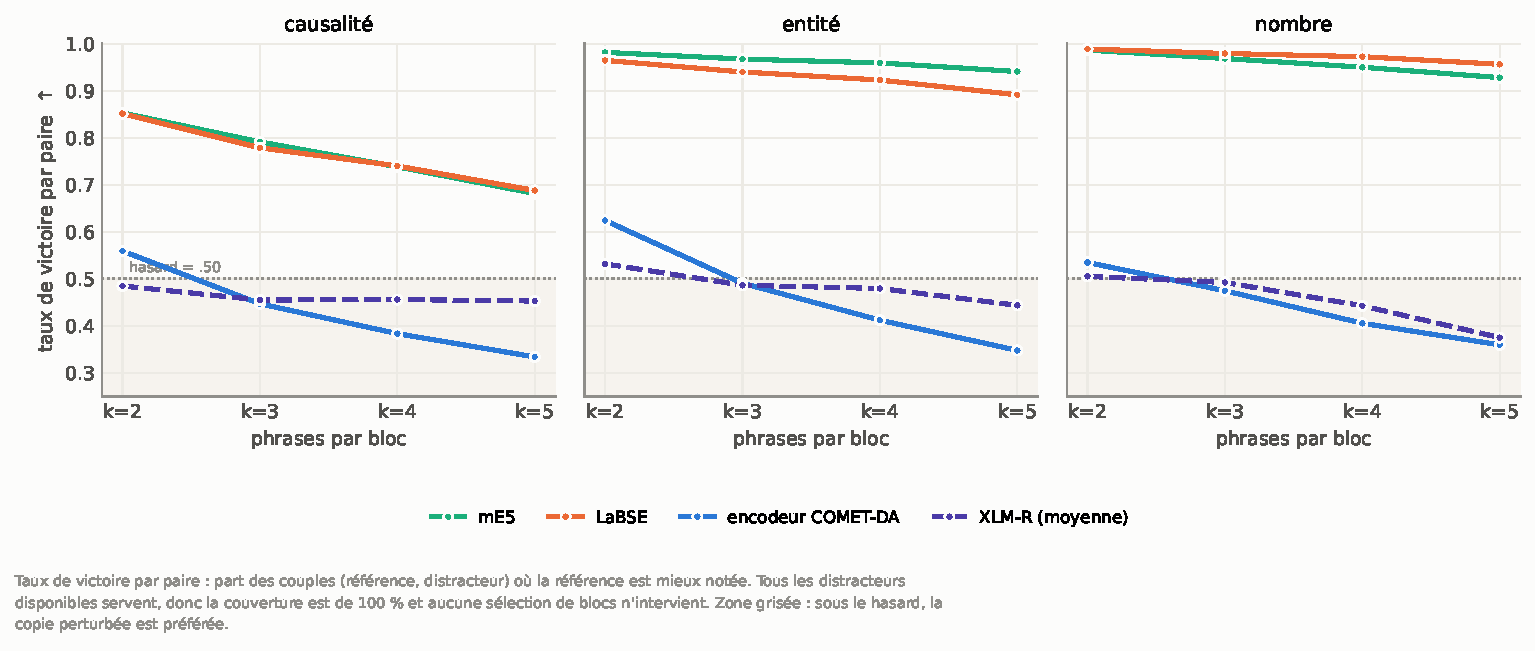
\includegraphics[width=\linewidth]{iso_by_category.pdf}
\caption{Taux de victoire par paire, par catégorie de perturbation. Zone grisée : sous le hasard, la copie perturbée est préférée.}
\label{fig:categorie}
\end{figure}

\begin{table}[t]
\centering\small
\begin{tabular}{l cccc cccc cccc}
\toprule
& \multicolumn{4}{c}{causalité} & \multicolumn{4}{c}{entité} & \multicolumn{4}{c}{nombre}\\
\cmidrule(lr){2-5}\cmidrule(lr){6-9}\cmidrule(lr){10-13}
encodeur & 2 & 3 & 4 & 5 & 2 & 3 & 4 & 5 & 2 & 3 & 4 & 5\\
\midrule
mE5               & .85 & .79 & .74 & .68 & .98 & .97 & .96 & .94 & .99 & .97 & .95 & .93\\
LaBSE             & .85 & .78 & .74 & .69 & .96 & .94 & .92 & .89 & .99 & .98 & .97 & .96\\
encodeur COMET-DA & .56 & .45 & .38 & .33 & .62 & .49 & .41 & .35 & .53 & .47 & .41 & .36\\
\quad + Bio-MQM   & .55 & .43 & .38 & .33 & .62 & .49 & .41 & .34 & .52 & .47 & .41 & .37\\
XLM-R (moyenne)   & .48 & .45 & .46 & .45 & .53 & .49 & .48 & .44 & .51 & .49 & .44 & .38\\
\bottomrule
\end{tabular}
\caption{Taux de victoire par paire, par catégorie et par longueur de bloc $k$ (colonnes 2 à 5). Hasard $=.50$. Couverture 100~\% : tous les distracteurs disponibles participent.}
\label{tab:categorie}
\end{table}

\subsection{Écarts entre langues}

Les moyennes cachent une dispersion importante pour COMET.
À $D=4$ et $k=2$, son taux de réussite vaut $.38$ en espagnol, $.17$ en français, $.16$ en russe et $.13$ en allemand.
L'écart est bien plus faible pour LaBSE ($.67$ à $.79$) et pour mE5 ($.76$ à $.83$).
Une part de cet écart tient à l'allemand, où la banque d'entités est plus bruitée : l'allemand met une majuscule à tous les noms communs, ce qui rend la frontière entre nom et entité nommée moins nette.
Les conclusions ne changent pas d'une langue à l'autre, mais les valeurs absolues à une seule langue ne doivent pas être citées seules.

\section{Aligner avec le score COMET plutôt qu'avec le cosinus}

\subsection{Ce que nous changeons}

Tout ce qui précède mesure un \emph{encodeur}.
Or ce que les utilisateurs rapportent n'est pas un encodeur, c'est une métrique : un encodeur \emph{plus} une tête de régression entraînée sur du jugement humain.

Nous gardons donc les mêmes articles, les mêmes blocs, les mêmes distracteurs, et nous ne changeons que la règle de décision :
\begin{align*}
\text{cosinus :} \quad & \arg\max_c \; \cos\big(\mathrm{plong}(\text{bloc source}), \mathrm{plong}(c)\big),\\
\text{score :} \quad & \arg\max_c \; \mathrm{COMET}(\text{src} = \text{bloc source},\ \text{mt} = c).
\end{align*}
La référence retenue est celle qui obtient le score le plus élevé.

Une contrainte s'impose : la règle du score exige une métrique \emph{sans référence}.
Au moment de l'alignement, la référence est justement ce qu'il faut retrouver ; la passer au modèle reviendrait à lui donner la réponse.
Nous utilisons donc \kiwi{} \citep{rei2022cometkiwi} pour la règle du score, et \cometda{} participe par la règle du cosinus, qui est celle où il était déjà.

Ce protocole utilise $D=2$ distracteurs, ce qui permet d'inclure $k=1$ : une phrase isolée n'admet souvent pas quatre perturbations distinctes.
La couverture vaut 87~\% à $k=1$ et atteint 100~\% dès $k=2$.
Le point $k=1$ est donc le seul à porter sur un sous-ensemble des blocs, et ce sous-ensemble est le plus riche en perturbations : une partie de la pente entre $k=1$ et $k=2$ vient de ce changement d'échantillon, pas du modèle.

\subsection{Résultat}

Le contraste est frappant (figure~\ref{fig:cometscore}, tableau~\ref{tab:comet}).

Le \textbf{score} CometKiwi réussit l'alignement dans $98$ à $99~\%$ des cas, à toutes les longueurs.
Son rang moyen reste à $1{,}01$--$1{,}02$ pour un hasard à $2{,}0$.
La courbe est plate : entre $k=1$ et $k=5$, la perte est de un point.

Le \textbf{cosinus} de l'encodeur COMET-DA, sur exactement les mêmes décisions, tombe de $.73$ à $.23$, et son rang moyen passe de $1{,}33$ à $2{,}17$, donc au-delà du hasard à partir de $k=4$.

L'explication est architecturale, et elle mérite d'être dite clairement.
La règle du cosinus compresse chaque côté en un vecteur unique, puis compare les deux vecteurs.
Un mot changé dans un bloc de cinq phrases ne déplace presque pas ce vecteur.
La règle du score, elle, donne les deux textes ensemble au modèle, qui les met en relation token par token par attention croisée avant de produire un nombre.
Le signal de l'erreur n'a jamais à survivre à une moyenne.

La conclusion est donc double, et il faut garder les deux moitiés.
La représentation \emph{pooled} de COMET perd l'erreur dès que le texte s'allonge.
La métrique complète, elle, la garde.
Le déficit constaté aux sections précédentes est un déficit de la représentation lue par un cosinus, pas une preuve que la métrique publiée est aveugle aux erreurs dans un texte long.

Une réserve enfin : à $D=2$, le score plafonne dès $k=1$.
La tâche est trop facile pour cette règle et ne permet pas de mesurer une pente.
Un protocole à $D$ plus grand, ou avec des perturbations plus subtiles, serait nécessaire pour situer le point de rupture du score.

\begin{figure}[t]
\centering
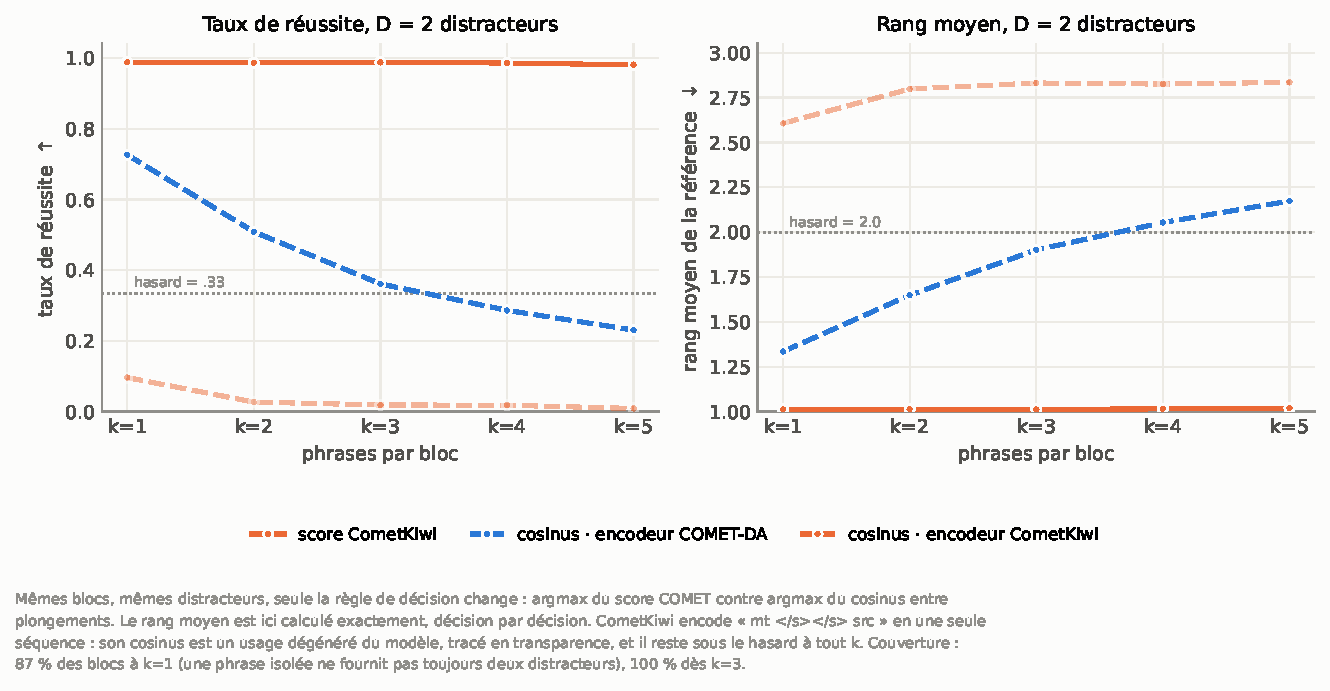
\includegraphics[width=\linewidth]{iso_comet_score.pdf}
\caption{Alignement par le score COMET contre alignement par le cosinus de l'encodeur, sur les mêmes blocs et les mêmes distracteurs, avec $D=2$. Le rang moyen est ici calculé exactement, décision par décision. La courbe transparente est le cosinus de CometKiwi : ce modèle encode « mt </s></s> src » en une seule séquence et n'a donc pas d'encodeur de texte isolé ; son cosinus est un usage dégénéré du modèle et reste sous le hasard partout.}
\label{fig:cometscore}
\end{figure}

\begin{table}[t]
\centering\small
\begin{tabular}{l ccccc ccccc}
\toprule
& \multicolumn{5}{c}{taux de réussite $A(2)$ $\uparrow$} & \multicolumn{5}{c}{rang moyen $R(2)$ $\downarrow$}\\
\cmidrule(lr){2-6}\cmidrule(lr){7-11}
règle de décision & $k{=}1$ & 2 & 3 & 4 & 5 & $k{=}1$ & 2 & 3 & 4 & 5\\
\midrule
score \kiwi{}                  & .99 & .99 & .99 & .99 & .98 & 1.01 & 1.01 & 1.01 & 1.02 & 1.02\\
cosinus, encodeur \cometda{}   & .73 & .51 & .36 & .29 & .23 & 1.33 & 1.65 & 1.90 & 2.05 & 2.17\\
cosinus, encodeur \kiwi{}$^\dagger$ & .10 & .03 & .02 & .02 & .01 & 2.61 & 2.80 & 2.83 & 2.83 & 2.84\\
\midrule
\emph{hasard} & .33 & .33 & .33 & .33 & .33 & 2.00 & 2.00 & 2.00 & 2.00 & 2.00\\
\bottomrule
\end{tabular}
\caption{Aligner avec le score plutôt qu'avec le cosinus, $D=2$ distracteurs, moyenne sur de/es/fr/ru. Le rang est exact ici. $^\dagger$ usage dégénéré : CometKiwi n'a pas d'encodeur de texte isolé.}
\label{tab:comet}
\end{table}

\section{Limites}

Nous listons ce qui doit accompagner ces nombres.

\begin{enumerate}
\item \textbf{Les blocs longs sont rares.} À $k=5$ il ne reste que 141 blocs par langue. L'intervalle de confiance binomial y est de l'ordre de $\pm.05$. Les pentes sont nettes, les valeurs individuelles le sont moins.
\item \textbf{Exiger $D$ distracteurs sélectionne les blocs.} La couverture est reportée systématiquement. Un point sous 80~\% de couverture n'est pas comparable à un point à 100~\%.
\item \textbf{Le rang du tableau~\ref{tab:principal} est reconstruit.} Il suppose un taux de victoire par paire homogène entre blocs. Le rang exact n'est disponible que pour le protocole à $D=2$ (tableau~\ref{tab:comet}).
\item \textbf{Le protocole à $D=2$ favorise les premières positions.} Les deux distracteurs retenus sont les deux de plus petit indice dans le vivier échantillonné, ce qui sur-représente les perturbations en début de bloc. La ventilation par paire, elle, utilise tous les distracteurs et ne souffre pas de ce biais.
\item \textbf{Les perturbations sont automatiques.} Elles ne sont pas validées à la main. Une perturbation « entité » peut produire une phrase sémantiquement étrange mais grammaticale ; c'est acceptable pour la tâche, mais ce n'est pas une erreur de traduction réaliste.
\item \textbf{Deux générateurs existent.} Le générateur spaCy et le générateur heuristique produisent des distracteurs différents. Les exécutions ne sont pas comparables entre générateurs. Tous les nombres de ce rapport viennent du générateur spaCy.
\item \textbf{Une seule direction.} Seul en$\to$xx est mesuré, avec quatre langues cibles européennes. Rien n'est établi pour xx$\to$en, ni pour les paires sans anglais, ni pour les langues à faibles ressources.
\end{enumerate}

\section{Reproduction}

Tout le protocole tient dans deux points d'entrée Python.
Les scripts Slurm ne font que fixer l'environnement.

\paragraph{Prérequis.}
FLORES+ est un jeu de données à accès contrôlé : il faut être authentifié sur le Hub Hugging Face et avoir accepté les conditions de \code{openlanguagedata/flores\_plus}.
Le générateur spaCy demande les petits modèles de chaque langue :
\begin{verbatim}
pip install spacy nltk
python -m spacy download de_core_news_sm   # es / fr / ru / en de meme
python -c "import nltk; nltk.download('wordnet'); nltk.download('omw-2.0')"
\end{verbatim}

\paragraph{Résultats par encodeur, $D \in \{4,5,6\}$.}
\begin{verbatim}
python experiments/length_isolation/run_duel.py \
  --encoders comet:Unbabel/wmt22-comet-da hf-mean:xlm-roberta-large labse e5 \
  --langs de es fr ru --pivot en --direction en2xx \
  --k_list 2 3 4 5 --splits dev devtest \
  --duel_sizes 6 5 4 --perturb_backend spacy --seed 42 \
  --flores_source plus \
  --output results/block_duel/block_duel.json
\end{verbatim}
Le cinquième encodeur du tableau~\ref{tab:principal} est un point de contrôle local issu de la partie~2 ; on l'ajoute avec \code{comet:<chemin>/last.ckpt}.
L'option \code{--dry\_run} affiche la couverture par $k$ et par $D$ sans charger de modèle, ce qui permet de vérifier le tableau~\ref{tab:donnees} sur CPU.

\paragraph{Score COMET contre cosinus, $D=2$.}
\begin{verbatim}
python experiments/length_isolation/run_comet_align.py \
  --scorers comet-score:Unbabel/wmt22-cometkiwi-da \
            encoder-cos:Unbabel/wmt22-cometkiwi-da \
            encoder-cos:Unbabel/wmt22-comet-da \
  --langs de es fr ru --k_list 1 2 3 4 5 --splits dev devtest \
  --negatives_per_block 6 --shortlist_size 3 \
  --perturb_backend spacy --seed 42 \
  --output results/comet_align/comet_align.json
\end{verbatim}

\paragraph{Figures.}
\begin{verbatim}
python report/figures/make_isolation_figures.py
\end{verbatim}
Ce script lit les deux fichiers JSON ci-dessus et écrit les figures de cette partie dans \code{report/figures/isolation/}.

\paragraph{Déterminisme.}
Avec la même graine, la même version des modèles spaCy et la même version de FLORES+, les distracteurs sont identiques d'une exécution à l'autre.
Les plongements sont mis en cache sur disque, indexés par (encodeur, ensemble exact de textes) : ajouter un encodeur ne recalcule que celui-là.

\section{Ce que cette partie établit}

Trois points, en une phrase chacun.

La longueur seule dégrade la capacité d'un encodeur à repérer une erreur locale, et cette dégradation est monotone en $k$ à nombre de candidats constant.

L'encodeur de COMET passe sous le hasard dès trois phrases concaténées, son squelette XLM-R y est déjà à deux, tandis que LaBSE et mE5 restent largement au-dessus jusqu'à cinq.

La tête de régression, elle, ne perd presque rien : le déficit est celui de la représentation compressée, et non celui de la métrique complète.

La partie suivante examine ce que l'ajustement de domaine change à cette représentation, et la partie~3 demande si un entraînement sur des textes plus longs la répare.

% ============================================================================
\bibliographystyle{plainnat}
\bibliography{references}

\end{document}
